\documentclass[11pt,a4paper]{article}

\usepackage[margin=1in]{geometry}
\usepackage[T1]{fontenc}
\usepackage{lmodern}
\usepackage{amsmath,amssymb}
\usepackage{booktabs}
\usepackage{graphicx}
\usepackage{caption}
\usepackage{subcaption}
\usepackage{hyperref}
\usepackage[numbers,sort&compress]{natbib}
\usepackage{url}

\hypersetup{
  colorlinks=true,
  linkcolor=black,
  citecolor=blue,
  urlcolor=blue
}

\title{Safety-Aware Evaluation of Classical and Deep Sequence Models for Turbofan Engine RUL Prediction on C-MAPSS}
\author{Ethan Huang\\Beihang University}
\date{June 25, 2026}

\begin{document}
\maketitle

\begin{abstract}
Remaining Useful Life (RUL) prediction is a core task in prognostics and health management for turbofan engines. Most benchmark comparisons emphasize aggregate regression accuracy, but maintenance decisions are safety-asymmetric: overestimating RUL can delay intervention, while underestimation is usually conservative but costly. This paper evaluates classical machine-learning pipelines and deep sequence pipelines on the NASA C-MAPSS FD001 and FD003 subsets under both standard and safety-oriented metrics. Ridge regression, Random Forest, Gradient Boosting, LSTM, GRU, and 1D-CNN models are compared using leakage-controlled preprocessing, engine-level validation splitting, capped RUL labels, and three random seeds. Focused GRU ablations evaluate longer input windows, increased hidden capacity, and a lightweight safety-aware loss. Results show that tree ensembles remain strong, especially on FD001, while a 50-cycle GRU achieves the best FD003 aggregate RMSE among the evaluated configurations. Safety-aware GRU training improves FD001 late-life performance and reduces FD003 overestimation frequency, but does not dominate all metrics. The study argues that C-MAPSS RUL evaluation should report not only RMSE and MAE, but also critical-zone error and overestimation behavior. The claims are intentionally scoped to FD001/FD003 and should be read as a reproducible student research benchmark rather than a new state-of-the-art method.
\end{abstract}

\noindent\textbf{Keywords:} Remaining Useful Life; C-MAPSS; turbofan engine; prognostics and health management; GRU; safety-aware loss

\section{Introduction}

Remaining Useful Life (RUL) prediction is a central task in prognostics and health management (PHM), where degradation signals are used to estimate how many operating cycles remain before failure. For safety-critical assets such as turbofan engines, prediction quality cannot be judged only by average numerical accuracy. A model that underestimates RUL may cause premature maintenance, additional cost, and reduced availability, whereas a model that overestimates RUL may delay intervention and expose the system to elevated operational risk. This asymmetry motivates evaluation protocols that distinguish general regression error from safety-relevant error patterns.

This study investigates RUL prediction on the NASA C-MAPSS turbofan engine simulation benchmark, distributed through the NASA Prognostics Center of Excellence data repository \citep{NASA_PCoE}. The benchmark has been widely used since the PHM data challenge and related dataset release \citep{Saxena2008}. In this work, the experimental scope is limited to FD001 and FD003. FD001 represents a single operating condition with a single fault mode, while FD003 represents a single operating condition with two fault modes. This contrast makes the pair useful for examining how model behavior changes when the degradation setting becomes more complex while the operating condition remains fixed. Importantly, the dataset is treated here as a simulation benchmark rather than as direct real-engine fleet data.

The goal of the paper is not to introduce a new state-of-the-art architecture. Instead, it provides a safety-aware evaluation of classical tree-based regressors and deep sequence models, including LSTM, GRU, and CNN variants. Standard metrics such as RMSE and MAE remain necessary because they summarize global predictive accuracy and allow comparison with prior work. However, they are insufficient for understanding whether a model is conservative or risk-seeking near end of life. Therefore, this study also emphasizes the NASA scoring function, critical-zone RMSE, and overestimation ratio. These metrics are used to characterize whether errors concentrate in late-life regions and whether models tend to predict more remaining life than is actually available.

The paper further examines whether two design choices improve GRU behavior: longer temporal windows and a safety-aware loss. Longer windows may expose the recurrent model to more degradation history, but they may also increase training difficulty and reduce the number of available training samples. A safety-aware loss can explicitly penalize hazardous overestimation, but it may trade global accuracy for more conservative predictions. Evaluating these choices under both FD001 and FD003 helps separate architecture-level effects from dataset-condition effects.

The contributions of this paper are:
\begin{enumerate}
    \item It presents a controlled practical pipeline comparison of classical feature-engineered models and deep sequence models for C-MAPSS FD001 and FD003 RUL prediction under both conventional and safety-oriented metrics.
    \item It evaluates safety asymmetry through NASA S-score, critical-zone RMSE, and overestimation ratio, with particular attention to the higher operational risk of RUL overestimation.
    \item It studies whether longer input windows and safety-aware loss improve GRU behavior within the evaluated single-operating-condition simulation scenarios.
\end{enumerate}

\section{Related Work}

The C-MAPSS dataset has become a standard benchmark for turbofan engine RUL prediction because it provides multivariate run-to-failure trajectories under controlled simulation settings \citep{NASA_PCoE,Saxena2008}. Each engine unit is observed over time through operational settings and sensor measurements, and the learning task is to estimate the remaining cycles before failure. The benchmark is commonly divided into subsets with different operating conditions and fault modes. FD001 is often used as a simpler starting point because it contains one operating condition and one fault mode. FD003 keeps the single operating condition but introduces two fault modes, making the degradation pattern more heterogeneous. This structure supports comparative studies that test whether a method remains reliable as fault complexity increases.

Early and classical approaches to RUL prediction often rely on engineered features, degradation indicators, or regression models trained on windowed sensor statistics. Tree-based models are attractive in this setting because they can model nonlinear feature interactions, handle mixed feature scales, and provide strong tabular baselines without requiring sequence-specific training. However, when temporal degradation patterns are important, fixed-window summaries may discard ordering information. For this reason, classical models are useful baselines but should be compared against architectures that directly process time-series sequences.

Deep learning methods address this limitation by learning representations from ordered sensor windows. Convolutional neural networks have been applied to RUL prediction by treating multivariate sensor histories as structured temporal inputs, allowing local degradation patterns to be extracted automatically \citep{Babu2016}. Recurrent models such as LSTM and GRU are also natural choices because they maintain hidden states across time and can capture longer temporal dependencies; LSTM-based RUL estimation has been specifically studied on prognostic sequence data \citep{Zheng2017}. Recent comparative work continues to evaluate classical and deep models on C-MAPSS-style RUL prediction tasks, reflecting that model choice remains sensitive to preprocessing, window length, subset difficulty, and evaluation protocol \citep{Goel2026}.

A recurring issue in this literature is that ranking models by RMSE or MAE alone may obscure safety-relevant behavior. In maintenance planning, an optimistic RUL estimate can be more dangerous than a pessimistic one. A model that predicts an engine has many cycles remaining when failure is near may delay inspection or replacement. Conversely, underestimation usually leads to earlier maintenance, which is costly but generally safer. The NASA scoring function partly captures this asymmetry by penalizing late predictions differently from early predictions, making it more aligned with prognostic risk than symmetric errors alone. Critical-zone metrics add another layer by focusing evaluation on the late-life region where decisions are most consequential.

This paper is positioned within that evaluation-oriented line of work. Rather than proposing a new architecture, it compares established model families under a consistent pipeline and reports both global accuracy and safety-aware indicators. This framing is especially important for FD001 and FD003: a method that performs acceptably under the simpler single-fault setting may not preserve the same error profile when two fault modes are present. By examining tree models, CNNs, LSTMs, GRUs, long-window GRUs, and safety-aware GRUs together, the study aims to provide an engineering-focused view of which modeling choices are accurate, which are conservative, and which may require caution before being used in safety-sensitive prognostic workflows.

\section{Methodology}

\subsection{Data Preparation}

This study evaluates RUL prediction on the NASA C-MAPSS turbofan degradation benchmark, using FD001 and FD003. FD001 represents a single operating condition with a single fault mode, whereas FD003 keeps the same single-condition setting but includes two fault modes. Each engine trajectory is treated as a multivariate time series indexed by cycle, and the prediction target is the RUL at the end of each input window.

\begin{table}[htbp]
\centering
\caption{Dataset scope used in this paper. Train engines are split into fitting and validation engines by unit ID. Test evaluation uses the final window of each test engine.}
\label{tab:dataset-scope}
\begin{tabular}{lrrrr}
\toprule
Subset & Operating conditions & Fault modes & Train/Test engines & Validation split \\
\midrule
FD001 & 1 & 1 & 100 / 100 & 20\% of train engines \\
FD003 & 1 & 2 & 100 / 100 & 20\% of train engines \\
\bottomrule
\end{tabular}
\end{table}

For training trajectories, the uncapped RUL at cycle $t$ of engine $u$ is computed from the final observed cycle $T_u$. Following the common piecewise-linear labeling protocol, the target is capped at a maximum RUL of 130 cycles:
\begin{equation}
y_{u,t} = \min(T_u - t, R_{\max}), \qquad R_{\max}=130.
\end{equation}
This cap prevents early-life samples from dominating the regression objective with large RUL values while preserving the degradation-sensitive low-RUL region.

Train and validation splits are performed by engine ID, so that windows from the same engine do not appear in both sets. The default validation fraction is 0.2, giving approximately 80 fitting engines and 20 validation engines for each subset and seed. Candidate channels include the three operating settings and 21 sensor channels. Low-variance columns are removed using the fitting split only, with variance threshold \(10^{-10}\). Feature scaling is fit only on the fitting engines and then applied unchanged to validation and test engines. This avoids validation or test leakage through normalization statistics. Unless otherwise specified, sequence models use sliding windows of 30 cycles and stride 1. A focused ablation also evaluates a longer 50-cycle window. For the test set, one prediction is produced per test engine by using the last available window, matching the practical setting in which the most recent operating history is used to estimate current RUL.

For classical machine-learning models, each 30-cycle or 50-cycle window is converted into fixed-length statistical descriptors. For every input channel in a window, we compute the mean, standard deviation, last observed value, delta, and slope. These features summarize the local operating level, variability, terminal state, short-term change, and linear degradation trend.

\subsection{Models}

We compare classical regression baselines with deep sequence models. The traditional models are Ridge regression, Random Forest, and Gradient Boosting. These models operate on the statistical window features described above. Ridge regression provides a linear regularized baseline, while Random Forest and Gradient Boosting provide nonlinear tree-based baselines that can capture interactions among sensor summaries without requiring sequential architectures.

The deep models are LSTM, GRU, and 1D-CNN networks trained directly on multivariate windows. The recurrent models process the input cycle by cycle and use the final sequence representation for RUL regression. The 1D-CNN uses temporal convolution over the window to learn local degradation patterns. The default deep configuration uses hidden size 64, one layer, dropout 0.2, Adam optimization with learning rate $10^{-3}$, batch size 128, and early stopping. These settings are kept fixed across the main comparisons to isolate the effect of model class and dataset condition.

This comparison is best interpreted as a practical pipeline comparison rather than a pure architecture comparison. The classical models receive engineered window summaries, whereas the deep models receive ordered sequence windows. Therefore, a strong tree result should be read as evidence that feature-engineered classical baselines are competitive in this setting, not as proof that tree architectures are universally superior to sequence models.

In addition to the default configuration, focused configurations are evaluated to probe safety and capacity effects. On FD001, we include \texttt{safety\_w1p5\_h64\_l1\_w30}. On FD003, we include \texttt{window50\_h64\_l1}, \texttt{capacity\_h128\_l1\_w30}, and \texttt{safety\_w1p5\_h64\_l1\_w30}. These focused runs test whether longer temporal context, increased hidden capacity, or safety-aware weighting improves performance under the single-condition, dual-fault setting. Wider one-seed sweeps for learning rate, scheduler, two-layer GRU, and window size were also run as exploratory experiments; the paper emphasizes the three-seed configurations because they provide the minimum robustness check.

\begin{table}[htbp]
\centering
\caption{Main experimental protocol. Full command outputs and CSV summaries are stored in the project repository.}
\label{tab:protocol}
\begin{tabular}{ll}
\toprule
Component & Setting \\
\midrule
RUL label & Piecewise capped RUL, \(R_{\max}=130\) \\
Split & Engine-level train/validation split, validation fraction 0.2 \\
Scaling & StandardScaler fit on fitting engines only \\
Default window & 30 cycles, stride 1 \\
Test rule & Last available window per test engine \\
Seeds & 42, 43, 44 for main comparisons and selected focused runs \\
Ridge & \(\alpha=1.0\) \\
Random Forest & 300 trees, minimum leaf size 2 \\
Gradient Boosting & 300 trees, learning rate 0.05, max depth 3 \\
LSTM/GRU & hidden size 64, 1 layer, FC head 64--32--1 \\
1D-CNN & Conv1d 32/64 channels, kernel size 3, adaptive average pooling \\
Optimization & Adam, learning rate \(10^{-3}\), batch size 128 \\
Early stopping & Maximum 100 epochs, patience 10 \\
\bottomrule
\end{tabular}
\end{table}

\subsection{Safety-Aware Training Objective}

Standard regression losses treat underestimation and overestimation symmetrically. In prognostics, however, overestimating RUL can be safety-critical because it may delay maintenance beyond the actual degradation state. We therefore evaluate a safety-aware weighted loss that increases the contribution of low-RUL critical samples and overestimation errors.

Let $\hat{y}_i$ be the predicted RUL and $y_i$ the capped target for sample $i$. We define the squared error with a sample-dependent weight:
\begin{equation}
\mathcal{L}_{\mathrm{safety}}
=
\frac{1}{N}\sum_{i=1}^{N}
w_i(\hat{y}_i-y_i)^2 .
\end{equation}
The implemented safety loss uses additive weights for two conditions: the sample is in the critical RUL region, or the model overestimates RUL. Specifically,
\begin{equation}
w_i =
1
+(\alpha-1)\mathbb{I}(y_i \leq 50)
+(\beta-1)\mathbb{I}(\hat{y}_i > y_i).
\end{equation}
For the focused safety-aware configurations, \(\alpha=\beta=1.5\). A sample that is both critical and overestimated therefore receives weight 2.0. This formulation keeps the objective simple while emphasizing the two error regimes most relevant to maintenance risk: late-life degradation and unsafe optimistic predictions. It is an exploratory benchmark-level safety objective, not a validated maintenance cost model.

\subsection{Evaluation Metrics}

Model performance is evaluated with both conventional regression metrics and safety-oriented metrics. RMSE and MAE measure average prediction accuracy:
\begin{equation}
\mathrm{RMSE}
=
\sqrt{
\frac{1}{N}
\sum_{i=1}^{N}
(\hat{y}_i-y_i)^2
},
\end{equation}
\begin{equation}
\mathrm{MAE}
=
\frac{1}{N}
\sum_{i=1}^{N}
|\hat{y}_i-y_i|.
\end{equation}

We also report the NASA scoring function, or S-score, which penalizes asymmetric RUL errors and is commonly used for C-MAPSS evaluation. With \(d_i=\hat{y}_i-y_i\), positive error indicates RUL overestimation and receives the stronger penalty:
\begin{equation}
S = \sum_i s_i,\qquad
s_i =
\begin{cases}
\exp(-d_i/13)-1, & d_i < 0,\\
\exp(d_i/10)-1, & d_i \geq 0.
\end{cases}
\end{equation}

In addition, we compute critical RMSE on samples with true RUL no greater than 50 cycles, focusing evaluation on the late-life region:
\begin{equation}
\mathrm{RMSE}_{\mathrm{crit}}
=
\sqrt{
\frac{1}{|\mathcal{C}|}
\sum_{i \in \mathcal{C}}
(\hat{y}_i-y_i)^2
},
\qquad
\mathcal{C}=\{i:y_i \leq 50\}.
\end{equation}

Finally, we report the overestimation ratio, defined as the fraction of predictions that exceed the true RUL:
\begin{equation}
\mathrm{OverRatio}
=
\frac{1}{N}
\sum_{i=1}^{N}
\mathbb{I}(\hat{y}_i > y_i).
\end{equation}
Together, these metrics distinguish general accuracy from safety-relevant behavior. RMSE and MAE summarize global fit, the NASA S-score reflects benchmark-specific asymmetric penalties, critical RMSE measures degradation-end performance, and the overestimation ratio directly quantifies the frequency of optimistic RUL predictions.

\section{Results}

Figure~\ref{fig:model-comparison} summarizes the test performance averaged over three random seeds. Tables~\ref{tab:fd001-results} and~\ref{tab:fd003-results} report mean test metrics, with RMSE shown as mean \(\pm\) standard deviation for compactness; the accompanying CSV files contain mean, standard deviation, minimum, and maximum for every metric. On FD001, tree-based baselines were the strongest overall performers. Gradient Boosting achieved the lowest RMSE, \(12.81 \pm 0.38\), with MAE \(9.83\), \(\textit{S}\)-score \(247.46\), critical RMSE50 \(5.60\), and overestimation ratio \(0.607\). Random Forest was close in RMSE, \(13.01 \pm 0.57\), and obtained the lowest MAE among the reported FD001 models, \(9.62\), with \(\textit{S}\)-score \(258.65\), critical RMSE50 \(6.21\), and overestimation ratio \(0.617\). These results indicate that classical ensemble pipelines remain highly competitive for the single operating condition and single fault mode represented by FD001.

Among the deep sequence models on FD001, the safety-weighted GRU provided the best deep-learning result. The GRU safety-w1.5 variant reached RMSE \(13.99 \pm 0.26\), MAE \(10.01\), \(\textit{S}\)-score \(312.82\), critical RMSE50 \(4.94\), and overestimation ratio \(0.563\). Relative to the baseline GRU, which obtained RMSE \(15.27 \pm 0.64\), MAE \(11.33\), \(\textit{S}\)-score \(483.23\), critical RMSE50 \(5.71\), and overestimation ratio \(0.587\), safety weighting improved both average error and late-life critical error. However, it did not surpass Gradient Boosting or Random Forest on the main RMSE and MAE metrics. The LSTM obtained RMSE \(15.60 \pm 0.51\) and critical RMSE50 \(6.52\), while Ridge was weaker in global RMSE, \(16.92 \pm 0.11\), and especially weak in the critical region, with RMSE50 \(16.68\). The CNN configuration performed poorly on FD001, with RMSE \(22.47 \pm 1.17\) and critical RMSE50 \(25.42\).

FD003 showed a different pattern. The best RMSE was achieved by the GRU window50 model, with RMSE \(12.96 \pm 0.48\), MAE \(9.30\), \(\textit{S}\)-score \(319.96\), critical RMSE50 \(5.50\), and overestimation ratio \(0.533\). Gradient Boosting remained very close, with RMSE \(13.21 \pm 0.35\), MAE \(9.67\), \(\textit{S}\)-score \(311.85\), critical RMSE50 \(5.53\), and overestimation ratio \(0.573\). Random Forest achieved RMSE \(13.98 \pm 0.25\), MAE \(10.14\), \(\textit{S}\)-score \(343.90\), critical RMSE50 \(4.76\), and overestimation ratio \(0.583\). Thus, the top-performing methods on FD003 were split between a longer-history GRU and classical tree ensembles.

The focused ablations in Figure~\ref{fig:focused-ablation} suggest that sequence length and safety weighting affect different aspects of performance. The GRU window50 variant was strongest in FD003 global RMSE and MAE among the evaluated configurations. This should be interpreted as an observed result of the tested 20/30/50-cycle window sweep rather than a general proof that longer windows always help. The GRU safety-w1.5 model achieved RMSE \(14.07 \pm 1.24\), MAE \(9.96\), \(\textit{S}\)-score \(413.74\), critical RMSE50 \(5.25\), and overestimation ratio \(0.437\). Although this variant did not dominate RMSE or \(\textit{S}\)-score, it produced the lowest reported FD003 overestimation ratio among the compared configurations. The baseline GRU obtained RMSE \(15.24 \pm 1.45\) and critical RMSE50 \(6.19\), while the hidden128 variant reached RMSE \(14.35 \pm 1.48\), critical RMSE50 \(5.98\), and overestimation ratio \(0.577\). The CNN again underperformed, with RMSE \(23.76 \pm 0.42\) and critical RMSE50 \(24.91\).

\begin{figure}[htbp]
    \centering
    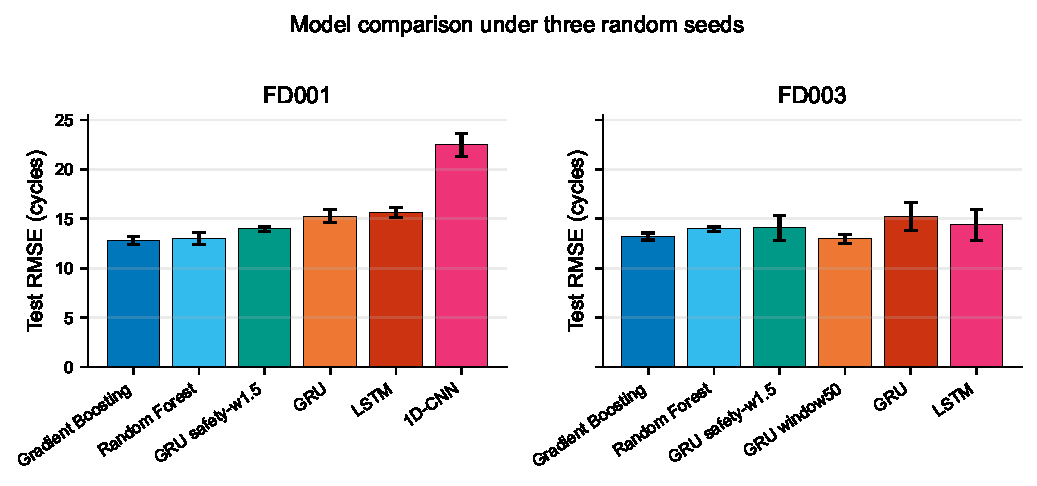
\includegraphics[width=\textwidth]{figures/figure_1_model_comparison.pdf}
    \caption{Model comparison under three random seeds. Bars show test RMSE means and error bars show standard deviations.}
    \label{fig:model-comparison}
\end{figure}

\begin{figure}[htbp]
    \centering
    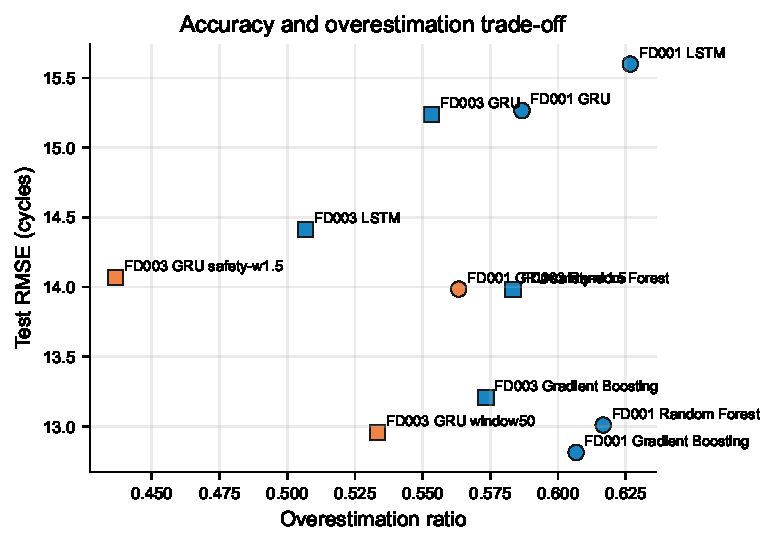
\includegraphics[width=0.82\textwidth]{figures/figure_2_safety_tradeoff.pdf}
    \caption{Accuracy and overestimation trade-off. Lower values on both axes are preferable; safety-aware GRU variants tend to reduce overestimation at the cost of not always minimizing RMSE.}
    \label{fig:safety-tradeoff}
\end{figure}

\begin{figure}[htbp]
    \centering
    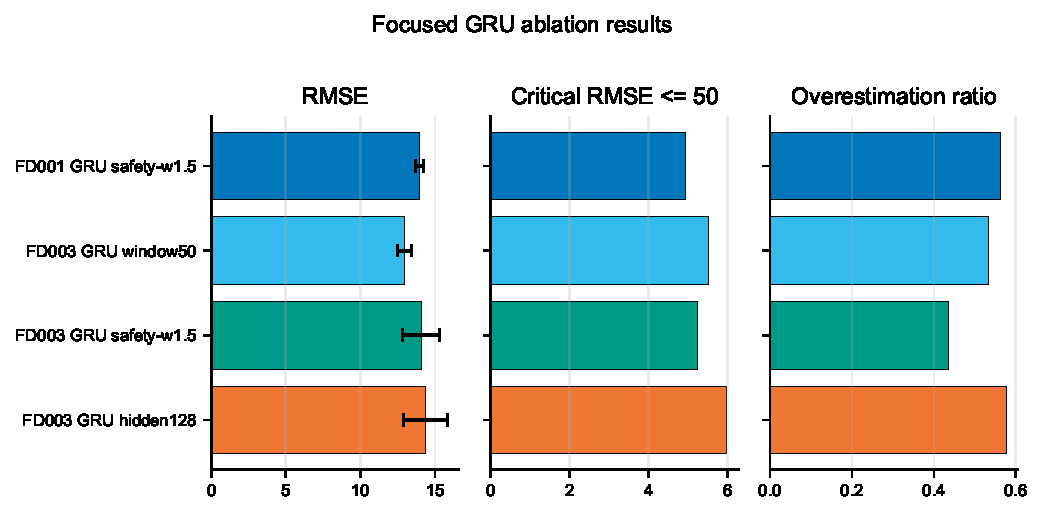
\includegraphics[width=\textwidth]{figures/figure_3_focused_ablation.pdf}
    \caption{Focused GRU ablation results for safety weighting, longer windows, and increased hidden capacity.}
    \label{fig:focused-ablation}
\end{figure}

\begin{table}[htbp]
\centering
\caption{Three-seed test results on FD001. Values are means across seeds, except RMSE which is shown as mean \(\pm\) standard deviation. Lower values are better except where noted.}
\label{tab:fd001-results}
\begin{tabular}{lrrrrr}
\toprule
Model & RMSE & MAE & S-score & RMSE50 & OverRatio \\
\midrule
Gradient Boosting & $12.81 \pm 0.38$ & 9.83 & 247.46 & 5.60 & 0.607 \\
Random Forest & $13.01 \pm 0.57$ & 9.62 & 258.65 & 6.21 & 0.617 \\
GRU safety-w1.5 & $13.99 \pm 0.26$ & 10.01 & 312.82 & 4.94 & 0.563 \\
GRU & $15.27 \pm 0.64$ & 11.33 & 483.23 & 5.71 & 0.587 \\
LSTM & $15.60 \pm 0.51$ & 11.45 & 563.57 & 6.52 & 0.627 \\
Ridge & $16.92 \pm 0.11$ & 13.33 & 510.32 & 16.68 & 0.580 \\
1D-CNN & $22.47 \pm 1.17$ & 16.49 & 3867.77 & 25.42 & 0.563 \\
\bottomrule
\end{tabular}
\end{table}

\begin{table}[htbp]
\centering
\caption{Three-seed test results on FD003. Focused GRU settings are included with the main baselines for comparison. Values are means across seeds, except RMSE which is shown as mean \(\pm\) standard deviation.}
\label{tab:fd003-results}
\begin{tabular}{lrrrrr}
\toprule
Model & RMSE & MAE & S-score & RMSE50 & OverRatio \\
\midrule
GRU window50 & $12.96 \pm 0.48$ & 9.30 & 319.96 & 5.50 & 0.533 \\
Gradient Boosting & $13.21 \pm 0.35$ & 9.67 & 311.85 & 5.53 & 0.573 \\
Random Forest & $13.98 \pm 0.25$ & 10.14 & 343.90 & 4.76 & 0.583 \\
GRU safety-w1.5 & $14.07 \pm 1.24$ & 9.96 & 413.74 & 5.25 & 0.437 \\
GRU hidden128 & $14.35 \pm 1.48$ & 10.48 & 407.65 & 5.98 & 0.577 \\
LSTM & $14.41 \pm 1.57$ & 10.22 & 550.26 & 5.09 & 0.507 \\
GRU & $15.24 \pm 1.45$ & 10.55 & 622.27 & 6.19 & 0.553 \\
Ridge & $18.02 \pm 0.37$ & 14.90 & 627.31 & 15.87 & 0.600 \\
1D-CNN & $23.76 \pm 0.42$ & 17.25 & 3533.32 & 24.91 & 0.570 \\
\bottomrule
\end{tabular}
\end{table}

\section{Discussion}

The main finding is that deep sequence models do not automatically outperform well-tuned classical baselines for turbofan RUL prediction. On FD001, Gradient Boosting and Random Forest were stronger than the GRU and LSTM variants on global error metrics. This is consistent with the structure of FD001: when the degradation process is relatively regular and the feature representation is informative, tree ensembles can model nonlinear sensor--RUL relationships effectively without requiring large amounts of sequence data or extensive representation learning. The result cautions against treating recurrent architectures as a default upgrade over classical baselines.

At the same time, the FD003 results show that deep sequence models can become more competitive when temporal history is better exploited. The GRU window50 model slightly outperformed Gradient Boosting in RMSE and MAE, while maintaining similar critical RMSE50. This supports a more conditional interpretation: recurrent models may benefit from longer historical context in this tested setting, but the advantage depends on model configuration and evaluation criterion. The difference between the baseline GRU and window50 GRU is therefore more informative than a broad comparison between ``deep'' and ``classical'' methods.

The safety-oriented results in Figure~\ref{fig:safety-tradeoff} further show that optimizing only for average RMSE is insufficient for maintenance-oriented RUL prediction. On FD001, safety-w1.5 improved the baseline GRU across RMSE, MAE, \(\textit{S}\)-score, critical RMSE50, and overestimation ratio. This is an important result because overestimated RUL can be operationally riskier than conservative underestimation. On FD003, safety-w1.5 did not produce the best RMSE, but it reduced the reported overestimation ratio to \(0.437\). This suggests a useful trade-off: safety weighting may shift the model toward more conservative predictions, although the gain in safety-sensitive behavior can come with weaker global ranking on RMSE or \(\textit{S}\)-score.

The CNN results should be interpreted narrowly. The current CNN configuration failed on both FD001 and FD003, especially in critical RMSE50. However, this does not imply that convolutional models are unsuitable for RUL prediction in general. It indicates that the tested CNN design, preprocessing, sequence length, or training setup was not effective in this experiment. Stronger temporal convolutional architectures, residual blocks, dilation, or hybrid CNN--RNN designs may behave differently.

\section{Threats to Validity}

Several threats to validity remain. First, three random seeds are a minimum robustness check, not a definitive statistical validation. Small differences, especially between GRU window50 and Gradient Boosting on FD003, should be treated cautiously until supported by more seeds or paired bootstrap confidence intervals over test engines. Second, FD001 and FD003 are both single-operating-condition subsets. The conclusions therefore apply to the evaluated FD001/FD003 setting, not to all C-MAPSS subsets or to real aircraft engine fleets. Third, the comparison mixes feature-engineered tabular pipelines and raw-sequence neural pipelines, which is useful for engineering practice but not a pure architecture ablation. Fourth, the safety-aware loss is intentionally simple and does not model an actual maintenance decision policy, uncertainty, or inspection cost.

\section{Limitations and Future Work}

Several limitations should be noted. First, the study reports results for FD001 and FD003 only. These subsets are useful because they contrast simpler and more complex degradation settings, but they do not cover the full C-MAPSS benchmark space. Future work should include FD002 and FD004 to evaluate robustness under multiple operating conditions.

Second, the comparison is limited to the tested configurations. The results support conclusions about these implementations, not about entire model families. Additional tuning of CNNs, recurrent architectures, feature selection, loss functions, and calibration methods may change the ranking. Third, although three-seed averages provide some stability, wider repeated trials and statistical testing would strengthen claims about small differences, especially between GRU window50 and Gradient Boosting on FD003.

Finally, the safety analysis uses overestimation ratio and critical RMSE50 as practical indicators, but real maintenance decisions may require cost-sensitive thresholds, uncertainty estimates, and decision-level simulation. Future work should connect predictive metrics to maintenance policies, false deferral costs, and conservative replacement trade-offs.

\section{Conclusion}

This study provides a safety-aware comparison of classical and deep sequence pipelines for turbofan RUL prediction on C-MAPSS FD001 and FD003. The results show that tree baselines remain strong, particularly on FD001, and that default deep sequence models do not automatically win. On FD003, the GRU window50 result suggests that longer temporal context can help recurrent models within the tested configurations. Safety weighting improved the GRU on FD001 and reduced FD003 overestimation frequency, but it did not dominate all metrics. Overall, RUL model selection should consider not only average accuracy, but also late-life error and the operational risk of overestimating remaining useful life.

\section*{Author Contributions}

Ethan Huang: conceptualization, software, data curation, experiments, visualization, analysis, and original draft preparation.

\section*{Data Availability}

The raw C-MAPSS files are publicly available from the NASA Prognostics Center of Excellence data repository \citep{NASA_PCoE}. The repository for this project does not redistribute the raw NASA data; experiment scripts and generated summaries are provided for reproducibility. Generated experiment tables are stored under \texttt{reports/tables/}, and the manuscript figures and summary table are stored under \texttt{reports/paper/}.

\section*{AI Disclosure}

This manuscript was prepared with assistance from AI-powered research and writing tools. The AI workflow supported experiment summarization, figure generation, draft organization, and editorial review simulation. The author directed the research question, executed the experiments locally, and is responsible for verifying all claims, citations, and conclusions before any formal submission.

\section*{Conflict of Interest}

The author declares no conflict of interest.

\section*{Funding}

This work received no external funding.

\bibliographystyle{plainnat}
\bibliography{references}

\end{document}
